



The next  model  used to identify the statistically significant factors affecting the time between successive renal function tests allows for only the level of renal function for each patient (as measured by their eGFR), and whether that test was analysed using the RenalQ system. In addition, the combination of these two effects has also been incorporated in the model. The regression model for this model yields  the following summary of effects and their statistical significance.
\begin{Schunk}
\begin{Soutput}
              Df    Deviance Resid. Df   -2*LL     Pr(>Chi)
NULL          NA          NA    246822 2250810           NA
System         1    81.24251    246821 2250729 1.996505e-19
EGFR_F        90 33987.39123    246731 2216742 0.000000e+00
System:EGFR_F 90   718.20686    246641 2216023 1.273500e-98
\end{Soutput}
\end{Schunk}


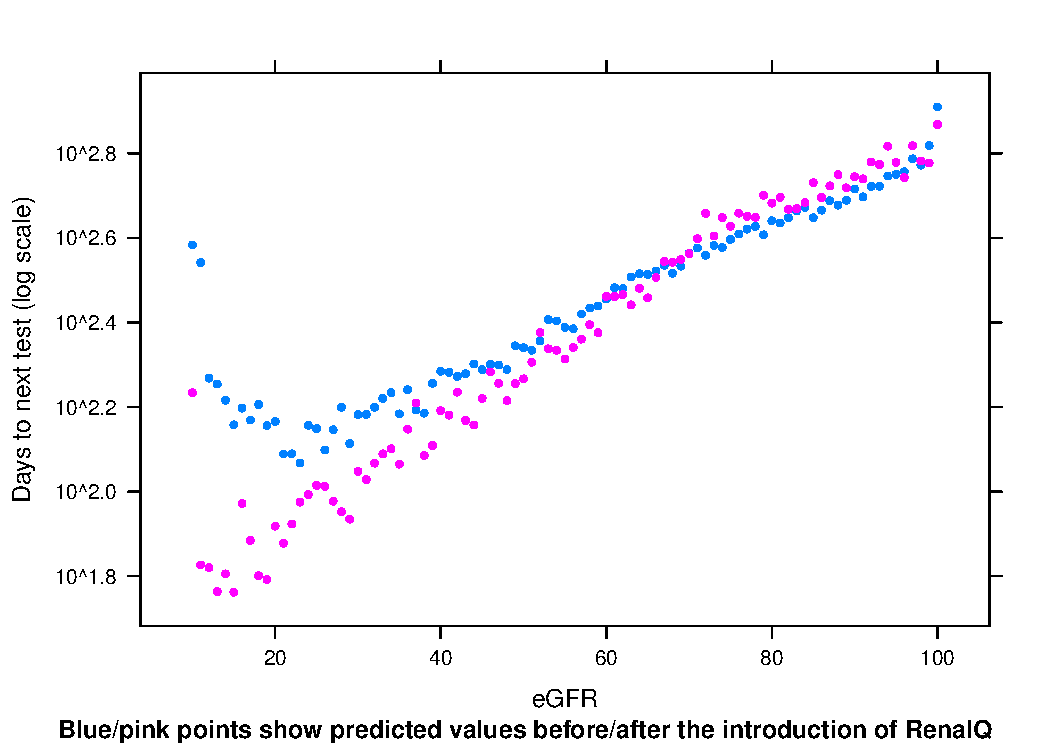
\includegraphics{Figures/RetestAll-ThePlots}

% This shows.
